\documentclass[tikz,border=3.14mm]{standalone}
\usepackage{tikz}

\begin{document}

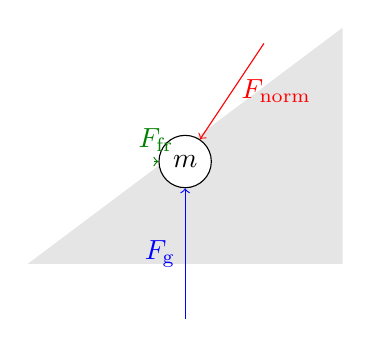
\begin{tikzpicture}
    % Draw inclined plane
    \fill[gray!20] (0,-1) -- (4,2) -- (4,-1) -- cycle;
    % Place object in middle
    \node[circle,draw,fill=white] (obj) at (2,0.3) {$m$};
    % Draw forces
    \draw[<-,blue] (obj)--++(0,-2) node[midway,left] {$F_{\mathrm{g}}$};
    \draw[<-,green!50!black] (obj)--++(-0.4,0) node[midway,above] {$F_{\mathrm{fr}}$};
    \draw[<-,red] (obj)--++(1,1.5) node[midway,right] {$F_{\mathrm{norm}}$};
\end{tikzpicture}

\end{document}